% !TEX program = pdflatex
% Informe Técnico — Proyecto Final TurtleBot 4 Lite (v2)
% Compilar:  pdflatex informe.tex  (2 pasadas)
% Figuras de resultados: python generar_figuras.py  (corre el simulador real del proyecto)
% Datos aún sin medir: \pend{...}  (texto rojo)
\documentclass[11pt,a4paper]{article}

\usepackage[utf8]{inputenc}
\usepackage[T1]{fontenc}
\usepackage[spanish,es-tabla,es-noshorthands]{babel}
\usepackage{lmodern}
\usepackage[a4paper,top=2.6cm,bottom=2.6cm,left=2.6cm,right=2.6cm,headheight=14pt]{geometry}
\usepackage{amsmath,amssymb}
\usepackage{graphicx}
\usepackage{booktabs,tabularx,array}
\usepackage[table]{xcolor}
\usepackage{tikz}
\usetikzlibrary{arrows.meta,positioning,shapes.geometric,fit,backgrounds,calc}
\usepackage{listings}
\usepackage{enumitem}
\usepackage{float}
\usepackage{microtype}
\usepackage{fancyhdr}
\usepackage[font=small,labelfont=bf,labelsep=period,format=hang,margin=8pt]{caption}
\usepackage[most]{tcolorbox}
\usepackage{hyperref}

\definecolor{azul}{HTML}{1F4E9C}
\definecolor{verde}{HTML}{2E8B57}
\definecolor{rojo}{HTML}{C0392B}
\hypersetup{colorlinks=true,linkcolor=azul,urlcolor=azul,citecolor=azul,
  pdftitle={Informe Técnico — TurtleBot 4 Lite},pdfauthor={Equipo Visión 67}}

\newcommand{\pend}[1]{\textcolor{rojo}{\textbf{[POR COMPLETAR: #1]}}}
\newcommand{\cmd}[1]{\texttt{\small #1}}

% Cuadros de texto
\newtcolorbox{decision}[1]{enhanced,breakable,colback=azul!4,colframe=azul,boxrule=0.6pt,
  arc=2pt,left=6pt,right=6pt,top=4pt,bottom=4pt,
  title={#1},fonttitle=\bfseries\small,coltitle=white,colbacktitle=azul,
  attach boxed title to top left={yshift=-2mm,xshift=4mm},boxed title style={arc=2pt}}
\newtcolorbox{leccion}[1]{enhanced,breakable,colback=verde!5,colframe=verde,boxrule=0.6pt,
  arc=2pt,left=6pt,right=6pt,top=4pt,bottom=4pt,
  title={#1},fonttitle=\bfseries\small,coltitle=white,colbacktitle=verde,
  attach boxed title to top left={yshift=-2mm,xshift=4mm},boxed title style={arc=2pt}}
\newtcolorbox{alerta}[1]{enhanced,breakable,colback=rojo!5,colframe=rojo,boxrule=0.6pt,
  arc=2pt,left=6pt,right=6pt,top=4pt,bottom=4pt,
  title={#1},fonttitle=\bfseries\small,coltitle=white,colbacktitle=rojo,
  attach boxed title to top left={yshift=-2mm,xshift=4mm},boxed title style={arc=2pt}}

% Encabezado y pie
\pagestyle{fancy}
\fancyhf{}
\fancyhead[L]{\small\textsc{Informe t\'ecnico --- TurtleBot 4 Lite}}
\fancyhead[R]{\small Equipo Visi\'on 67}
\fancyfoot[C]{\small\thepage}
\renewcommand{\headrulewidth}{0.4pt}
\setlength{\parskip}{3pt}
\renewcommand{\arraystretch}{1.12}
\setlist{itemsep=2pt,topsep=3pt}

\lstdefinestyle{codigo}{
  basicstyle=\ttfamily\footnotesize, numbers=left, numberstyle=\tiny\color{gray},
  frame=single, rulecolor=\color{gray!60}, breaklines=true, columns=fullflexible, keepspaces=true,
  keywordstyle=\color{azul}, commentstyle=\color{verde!70!black},
  stringstyle=\color{orange!70!black}, language=Python, showstringspaces=false,
  backgroundcolor=\color{gray!6}, xleftmargin=1.5em}
\lstset{style=codigo}

\tikzset{
  blk/.style={draw,rounded corners=2pt,align=center,font=\footnotesize,minimum height=8mm,inner sep=3pt,fill=#1},
  blk/.default=white,
  flecha/.style={-{Stealth[length=2mm]},thick},
  est/.style={draw,circle,align=center,font=\scriptsize,minimum size=14mm,inner sep=1pt,fill=blue!8}
}

\graphicspath{{figuras/}}
% generado por generar_figuras.py -- no editar a mano
\newcommand{\TablaCircuitos}{\begin{tabular}{@{}lrrrrc@{}}\toprule
\textbf{Circuito} & $t_{A\to B}$ (s) & $t_{\text{total}}$ (s) & Choques & Holgura m\'in.\ (cm) & Error en $A$ (cm)\\\midrule
Obstáculos en sala & 24,4 & 50,0 & 0 & 38,9 & 19,0\\
Laberinto con callejón & 51,6 & 104,0 & 0 & 14,8 & 20,2\\
Pasillo en L & -- & 300,1 & 0 & 14,6 & 171,2\\
Obstáculo bajo (invisible) & 31,5 & 53,2 & 0 & 83,4 & 19,7\\
\bottomrule\end{tabular}}
\newcommand{\TablaDeriva}{\begin{tabular}{@{}rcccc@{}}\toprule
\textbf{Deriva} & \textbf{ICP} & \textbf{Misiones OK} & \textbf{Error medio (cm)} & \textbf{Error m\'ax.\ (cm)}\\\midrule
0\,\% & no & 5/5 & 19,7 & 19,9\\
0\,\% & s\'i & 5/5 & 19,2 & 19,4\\
4\,\% & no & 5/5 & 39,4 & 44,4\\
4\,\% & s\'i & 5/5 & 19,1 & 19,3\\
8\,\% & no & 5/5 & 69,0 & 87,0\\
8\,\% & s\'i & 5/5 & 19,3 & 20,0\\
12\,\% & no & 5/5 & 92,5 & 103,6\\
12\,\% & s\'i & 5/5 & 19,3 & 20,0\\
\bottomrule\end{tabular}}
\newcommand{\TablaVelocidad}{\begin{tabular}{@{}rrrr@{}}\toprule
$v_{\max}$ (m/s) & Tiempo (s) & Choques & Holgura m\'in.\ (cm)\\\midrule
0,08 & 85,6 & 0 & 37,6\\
0,10 & 69,1 & 0 & 37,5\\
0,14 & 50,0 & 0 & 38,9\\
0,18 & 39,7 & 0 & 38,8\\
0,22 & 33,0 & 0 & 38,7\\
0,26 & 28,5 & 0 & 38,7\\
0,31 & 24,6 & 0 & 38,6\\
\bottomrule\end{tabular}}


\begin{document}

%=====================================================================
% PORTADA
%=====================================================================
\begin{titlepage}
\thispagestyle{empty}
\begin{tikzpicture}[remember picture,overlay]
  \fill[azul] (current page.north west) rectangle ($(current page.north east)+(0,-5.2cm)$);
  \fill[azul!60!white] ($(current page.north west)+(0,-5.2cm)$) rectangle ($(current page.north east)+(0,-5.5cm)$);
\end{tikzpicture}
\vspace*{0.4cm}
{\color{white}\Large\textsc{Proyecto final}\\[1mm]\large Rob\'otica m\'ovil y visi\'on por computador}\\[2.2cm]
\begin{flushleft}
{\Huge\bfseries\color{azul} Informe T\'ecnico}\\[5mm]
{\Large Navegaci\'on aut\'onoma, reconocimiento facial\\ y teleoperaci\'on por gestos con el\\ \textbf{TurtleBot~4 Lite}}\\[1.2cm]
\rule{0.35\textwidth}{1.2pt}\\[6mm]
{\large Plataforma: iRobot Create~3 + Raspberry~Pi~4 + RPLIDAR A1 + OAK-D Lite\\
Software: ROS~2 Jazzy, Fast~DDS, OpenCV, MediaPipe}
\end{flushleft}
\vfill
\noindent\begin{tabular}{@{}ll@{}}
\textbf{Equipo:} & Visi\'on 67 \\
\textbf{Integrantes:} & \pend{nombres y c\'odigos} \\
\textbf{Curso / docente:} & \pend{curso y docente} \\
\textbf{Fecha de entrega:} & 22 de noviembre de 2026 \\
\end{tabular}
\end{titlepage}

%=====================================================================
\pagenumbering{roman}
\begin{abstract}
\noindent Este informe cuenta c\'omo dise\~namos, y sobre todo \emph{por qu\'e} dise\~namos as\'i, el sistema que resuelve las dos tareas de la
competencia con el TurtleBot~4 Lite: (A)~ir de forma aut\'onoma de un punto $A$ a un punto $B$ en un circuito que no conocemos de antemano,
reconocer la foto de una persona contra una galer\'ia cargada sin internet, volver a $A$ y decir su nombre; y (B)~hacer lo mismo guiando al robot
solo con gestos de la mano.

La soluci\'on combina un navegador reactivo tipo VFH con memoria de ``migas de pan'' y correcci\'on de deriva por ICP~2D, un pipeline
YuNet\,+\,SFace para la cara y MediaPipe para la mano, coordinados por una m\'aquina de estados. Probamos el stack cl\'asico Nav2\,+\,SLAM y lo
descartamos porque la Raspberry~Pi no lo soporta junto con los sensores. Adem\'as de las pruebas en el laboratorio, corrimos el c\'odigo real
de navegaci\'on sobre un simulador de LiDAR; all\'i el ICP baja el error de regreso de 92~cm a 19~cm con una deriva de giro del 12\,\%. Tambi\'en
encontramos un caso que \textbf{todav\'ia falla} (un pasillo en L con la configuraci\'on conservadora final) y lo documentamos con honestidad.
Siguiendo el reglamento, el c\'odigo se reserva a los ap\'endices.
\end{abstract}
\vspace{4mm}
\tableofcontents
\clearpage
\listoffigures
\listoftables
\clearpage
\pagenumbering{arabic}

%=====================================================================
\section{Introducci\'on}
%=====================================================================
\subsection{Qu\'e nos pidieron}
\begin{description}[leftmargin=1.2cm,style=nextline]
\item[Tarea A (aut\'onoma).] El robot parte parado en la zona $A$, navega esquivando obst\'aculos y paredes hasta $B$, escanea con la OAK-D Lite
la fotograf\'ia de una persona y la compara con una galer\'ia \emph{offline}; luego regresa a $A$ y anuncia el nombre en voz alta. Nadie puede tocar nada.
\item[Tarea B (gestos).] Misma misi\'on, pero guiada por gestos frente a una c\'amara. Est\'an prohibidos el teclado, el mouse, el joystick y los
comandos por terminal durante el recorrido.
\end{description}

\subsection{La nota manda: c\'omo el puntaje moldea el dise\~no}
El puntaje de cada tarea es $P = 4.5\,\dfrac{t_{\max}-t}{t_{\max}-t_{\min}}$, con $t$ el tiempo total \emph{m\'as} las penalizaciones por choque
contra obst\'aculo o pared y por identificar mal a la persona. Si el robot no regresa a $A$, o si $t>t_{\max}$, el intento vale cero. Se permiten tres
intentos por tarea y cuenta el mejor.

\begin{decision}{Lo que esto significa para nosotros}
\begin{enumerate}[nosep]
\item \textbf{Fallar vale cero.} Un robot lento que vuelve sin chocar gana a uno veloz que se atasca. Primero completar, despu\'es acelerar.
\item \textbf{El circuito se revela el d\'ia de la prueba}, as\'i que no hay mapa previo ni entrenamiento con las personas objetivo. Necesitamos un
sistema reactivo y una galer\'ia que se cargue en segundos.
\end{enumerate}
\end{decision}

\subsection{Plataforma}
TurtleBot~4 Lite: base iRobot Create~3 (odometr\'ia, bumpers, buzzer), Raspberry~Pi~4 de 4~GB, LiDAR RPLIDAR~A1 (720 rayos, 0.15--12~m, unos 7.6~Hz
medidos) y c\'amara OAK-D Lite. El laboratorio es una red local \emph{sin internet} con tres robots compartidos; por eso todos los modelos de visi\'on
viajan ya descargados y cada robot usa su propio \texttt{ROS\_DOMAIN\_ID} (el nuestro es el 67).

\subsection{C\'omo leer este documento}
Primero el sistema completo (Secci\'on~\ref{sec:arq}), luego los dos m\'odulos de visi\'on (\ref{sec:vision}), la estrategia de navegaci\'on
(\ref{sec:nav}) y la justificaci\'on de cada decisi\'on (\ref{sec:just}). Los resultados (\ref{sec:result}) separan con cuidado lo que medimos en el robot,
lo que medimos en simulaci\'on y lo que todav\'ia falta; las limitaciones (\ref{sec:futuro}) incluyen un fallo real que encontramos al escribir este informe.

%=====================================================================
\section{Arquitectura general del sistema}
\label{sec:arq}
%=====================================================================
\subsection{Componentes y flujo de datos}
La Figura~\ref{fig:arq} muestra el sistema de punta a punta. Los sensores publican en ROS~2; los m\'odulos de percepci\'on y navegaci\'on consumen
\cmd{/scan}, \cmd{/odom}, la imagen de la OAK-D y \cmd{/hazard\_detection}; el coordinador de misi\'on decide en qu\'e etapa estamos; y el \'unico
actuador de movimiento es \cmd{/cmd\_vel} (m\'as \cmd{/cmd\_audio} para el buzzer).

\begin{figure}[H]
\centering
\begin{tikzpicture}[x=1cm,y=1cm,
  n/.style={blk=#1,text width=3.0cm,font=\scriptsize,minimum height=9mm},
  n/.default=white]
\node[n=orange!15] (lidar) at (0,0)    {RPLIDAR A1\\\texttt{/scan}};
\node[n=orange!15] (odom)  at (0,-1.5) {Create 3: odometr\'ia\\\texttt{/odom}};
\node[n=orange!15] (bump)  at (0,-3.0) {Create 3: bumpers\\\texttt{/hazard\_detection}};
\node[n=orange!15] (cam)   at (0,-4.5) {OAK-D Lite (RGB)\\\texttt{/oakd/.../compressed}};
\node[n=green!12] (vfh)   at (4.4,0)    {Evasi\'on VFH-lite\\(\texttt{nav\_core})};
\node[n=green!12] (migas) at (4.4,-1.5) {Migas + ICP 2D\\(memoria y regreso)};
\node[n=green!12] (face)  at (4.4,-3.0) {Reconocimiento facial\\YuNet + SFace};
\node[n=green!12] (hand)  at (4.4,-4.5) {Gestos de mano\\MediaPipe (Tarea B)};
\node[n=blue!12,minimum height=3.2cm] (fsm) at (8.6,-2.25) {\textbf{Coordinador de misi\'on}\\M\'aquina de estados\\(\texttt{mision.py})};
\node[n=green!12] (ctl) at (12.6,-0.9) {Control cinem\'atico\\rampas + guardi\'an};
\node[n=orange!15] (act) at (12.6,-2.7) {Create 3\\\texttt{/cmd\_vel}, buzzer};
\node[n=purple!10] (voz) at (12.6,-4.5) {Anuncio de voz\\(TTS en laptop)};
\draw[flecha] (lidar)--(vfh); \draw[flecha] (odom)--(migas); \draw[flecha] (bump)--(migas);
\draw[flecha] (cam)--(face); \draw[flecha] (cam)--(hand);
\draw[flecha] (lidar.south east)--(migas.north west);
\draw[flecha] (vfh.east)--(fsm.north west); \draw[flecha] (migas.east)--(fsm.west|-migas.east);
\draw[flecha] (face.east)--(fsm.west|-face.east); \draw[flecha] (hand.east)--(fsm.south west);
\draw[flecha] (fsm.east|-ctl.west)--(ctl.west); \draw[flecha] (ctl.south)--(act.north);
\draw[flecha] (fsm.east|-voz.west)--(voz.west);
\begin{scope}[on background layer]
\node[draw=gray,dashed,rounded corners,fit=(lidar)(cam),inner sep=5pt,label={[font=\footnotesize]above:Sensores}] {};
\node[draw=gray,dashed,rounded corners,fit=(vfh)(hand),inner sep=5pt,label={[font=\footnotesize]above:Percepci\'on y navegaci\'on}] {};
\node[draw=gray,dashed,rounded corners,fit=(ctl)(voz),inner sep=5pt,label={[font=\footnotesize]above:Actuaci\'on}] {};
\end{scope}
\end{tikzpicture}
\caption{Arquitectura de componentes. Naranja: hardware; verde: percepci\'on y navegaci\'on; azul: coordinaci\'on; morado: interacci\'on.}
\label{fig:arq}
\end{figure}

\subsection{Qu\'e corre en el robot y qu\'e en la laptop}
Armamos el software para que el \emph{mismo c\'odigo} corra en dos modalidades; as\'i podemos elegir seg\'un lo bueno que sea el enlace de red el d\'ia de la
competencia (Tabla~\ref{tab:computo}).

\begin{table}[H]
\centering\small
\begin{tabularx}{\textwidth}{@{}l>{\raggedright\arraybackslash}X>{\raggedright\arraybackslash}X@{}}
\toprule
 & \textbf{Onboard (Raspberry Pi 4 / Create 3)} & \textbf{Offboard (laptop, WSL2 + ROS 2)} \\
\midrule
Siempre & Drivers de LiDAR, c\'amara OAK-D e IMU; \emph{bridge} del Create~3; publicaci\'on de t\'opicos DDS & \\
Modalidad \emph{laptop} (por defecto) & \textbf{Solo retransmisi\'on de sensores} ($\approx$25\,\% de un n\'ucleo) &
Lazo de control $\texttt{/scan}\!\to\!\texttt{/cmd\_vel}$ a 20~Hz; YuNet+SFace; MediaPipe; m\'aquina de estados; voz \\
Modalidad \emph{edge} (\texttt{tarea\_*\_onboard.sh}) & Lazo de control y misi\'on completos en la Pi (inmune a cortes de red) &
Solo anuncio de voz y monitoreo \\
\bottomrule
\end{tabularx}
\caption{Reparto de c\'omputo entre el robot y la estaci\'on externa.}
\label{tab:computo}
\end{table}

La laptop y el robot se hablan por Fast~DDS en modo unicast con \emph{peers} est\'aticos (\texttt{fastdds\_pc.xml}); la imagen viaja siempre como
\cmd{/compressed}. Usamos Ethernet directo ($192.168.185.10 \leftrightarrow 192.168.185.3$, menos de 1~ms) o la red del laboratorio.

\begin{leccion}{Lo que nos cost\'o aprender de la red}
\begin{itemize}[nosep]
\item El Wi-Fi del campus bloquea el descubrimiento DDS: hay \emph{ping} y SSH, pero \cmd{ros2 topic list} sale casi vac\'io. Soluci\'on: la red del
laboratorio o cable.
\item Con peers est\'aticos, Fast~DDS contactaba solo cuatro participantes y faltaban t\'opicos; un perfil XML expl\'icito lo resolvi\'o.
\item \textbf{El reloj}: sin internet, la Pi y el Create~3 arrancan con fechas distintas y TF descarta mensajes (\emph{queue is full}). Sincronizamos la
Pi desde la laptop y reiniciamos el cliente NTP del Create~3; el desfase pas\'o de 75\,368~s (casi 21~h) a 0.08~s.
\end{itemize}
\end{leccion}

\subsection{C\'omo usamos cada sensor}
\begin{itemize}
\item \textbf{LiDAR RPLIDAR A1} (\cmd{/scan}): es el sensor principal para evitar obst\'aculos. Filtramos \texttt{inf}/\texttt{NaN} y rotamos el marco
angular para alinearlo con el frente del chasis. Alimenta la distancia libre, el margen lateral, el detector de concavidades y el ICP.
\item \textbf{Odometr\'ia del Create~3} (\cmd{/odom}): da la pose relativa a $A$ (se captura al inicio). Deriva por patinaje, as\'i que durante el
regreso la corregimos con ICP (Secci\'on~\ref{sec:retorno}).
\item \textbf{OAK-D Lite}: la usamos \'unicamente como c\'amara RGB (cara en $B$; opcionalmente se\~nales del circuito). Solo se decodifica cuando el estado
lo necesita, para cuidar la CPU. No usamos todav\'ia su profundidad est\'ereo (ver trabajo futuro).
\item \textbf{Bumpers del Create~3} (\cmd{/hazard\_detection}): \'ultima defensa contra obst\'aculos bajo el plano del LiDAR. Ojo: la base \textbf{no tiene
sensores traseros}, as\'i que retrocedemos despacio.
\end{itemize}

%=====================================================================
\section{Algoritmos de visi\'on por computador}
\label{sec:vision}
%=====================================================================
\subsection{Reconocimiento facial}
\label{sec:facial}
El problema es de \textbf{conjunto cerrado}: no se trata de decir ``qui\'en es'' entre millones, sino cu\'al de las personas de la galer\'ia es la de la foto.
La dificultad es la imagen: una foto \emph{impresa} vista por una c\'amara peque\~na (la vista previa de la OAK-D mide 250~px) con movimiento
residual. La Figura~\ref{fig:facial} resume el pipeline.

\begin{figure}[H]
\centering
\begin{tikzpicture}[n/.style={blk=#1,text width=2.6cm,font=\scriptsize}]
\node[n=gray!10]   (g)  at (0,0)    {Fotos de galer\'ia\\\texttt{galeria/Nombre/*.jpg}};
\node[n=blue!10]   (e1) at (3.6,0)  {Detecci\'on + alineaci\'on + embedding (original y espejo)};
\node[n=yellow!15] (c)  at (7.2,0)  {Cach\'e de galer\'ia\\\texttt{.cache.npz}};
\node[n=gray!10]   (f)  at (0,-2.2) {$N$ cuadros de la c\'amara en $B$};
\node[n=blue!10]   (d)  at (3.6,-2.2) {YuNet:\\caja + 5 puntos};
\node[n=blue!10]   (q)  at (7.2,-2.2) {Calidad $Q$ y selecci\'on de los mejores $K$};
\node[n=blue!10]   (s)  at (10.8,-2.2) {SFace:\\embedding 128-d};
\node[n=green!12]  (m)  at (10.8,-4.4) {Coseno contra galer\'ia\\(m\'ax. por persona)};
\node[n=green!12]  (r)  at (7.2,-4.4) {Decisi\'on:\\umbral $\tau$ + margen $\delta$};
\draw[flecha] (g)--(e1); \draw[flecha] (e1)--(c);
\draw[flecha] (f)--(d); \draw[flecha] (d)--(q); \draw[flecha] (q)--(s);
\draw[flecha] (s)--(m); \draw[flecha] (m)--(r);
\draw[flecha] (c.east) -- (12.9,0) |- (m.east);
\node[font=\scriptsize\itshape,anchor=south west] at (-1.3,0.65) {Offline (una vez)};
\node[font=\scriptsize\itshape,anchor=south west] at (-1.3,-1.55) {Online (en $B$)};
\end{tikzpicture}
\caption{Pipeline de reconocimiento facial. Arriba, lo que se hace una sola vez al cargar la galer\'ia; abajo, lo que ocurre en $B$.}
\label{fig:facial}
\end{figure}

\paragraph{1. Detecci\'on.} \textbf{YuNet} (OpenCV Zoo, formato ONNX) entrega, por cada cara, su caja, cinco puntos (ojos, nariz, comisuras de la boca) y una
confianza; descartamos detecciones con confianza menor a 0.6. Si la imagen es chica (lado mayor $<480$~px) la ampliamos con interpolaci\'on bic\'ubica. Si
hay varias caras elegimos la de mayor \'area.

\paragraph{2. Elegir los mejores cuadros.} En $B$ el robot acaba de frenar y la imagen puede estar movida. Por eso no confiamos en un solo cuadro:
puntuamos cada uno con
\[
  Q \;=\; c \cdot \min\!\left(\tfrac{w}{80},1\right)\cdot \min\!\left(\tfrac{\operatorname{Var}\!\left(\nabla^2 I_{\text{cara}}\right)}{100},1\right),
\]
donde $c$ es la confianza de YuNet, $w$ el ancho de la cara en p\'ixeles y $\operatorname{Var}(\nabla^2 I)$ la varianza del Laplaciano, una medida simple de
nitidez. Nos quedamos con los $K=3$ mejores.

\paragraph{3. Embedding.} Alineamos la cara con sus cinco puntos a $112\times112$ y \textbf{SFace} produce un vector de 128 dimensiones que normalizamos
a norma unitaria.

\paragraph{4. Matching.} Con vectores unitarios, la similitud coseno es un simple producto punto. Para la persona $p$, con embeddings de galer\'ia
$\mathcal{G}_p$ (incluyendo la versi\'on espejada de cada foto) y los $K$ mejores cuadros $\{e_k\}$:
\[
  s_p \;=\; \frac{1}{K}\sum_{k=1}^{K}\;\max_{g\in\mathcal{G}_p}\; e_k\!\cdot g, \qquad \hat p=\arg\max_p s_p .
\]
Tomamos el \emph{m\'aximo} por persona porque basta con que una foto de la galer\'ia se parezca a la entrada, y \emph{promediamos} entre cuadros para
reducir el ruido.

\paragraph{5. Decisi\'on.} El resultado es \emph{seguro} si $s_{\hat p}\ge\tau=0.363$ (umbral recomendado por OpenCV para SFace) y si la ventaja sobre el
segundo es al menos $\delta=0.04$. Si nadie supera el umbral devolvemos igual al m\'as parecido: en la competencia responder algo es mejor que no responder,
y la marca \emph{seguro} solo sirve para decidir si repetimos el barrido.

\paragraph{6. Galer\'ia y arranque.} Los embeddings se guardan en un cach\'e indexado por ruta, fecha y tama\~no del archivo, as\'i que cargar una galer\'ia
nueva el d\'ia de la prueba toma segundos. Tambi\'en hacemos una inferencia ``en vac\'io'' en $A$ (\emph{warm-up}): la primera inferencia de OpenCV DNN es mucho m\'as
lenta y, si cayera en $B$, nos costar\'ia tiempo. El modo \emph{deja-uno-fuera} (\cmd{facial.py --probar}) estima la precisi\'on sobre la propia galer\'ia y
avisa de fotos donde no se detecta cara.

\paragraph{7. Si no se ve la cara.} El robot barre girando a $0.4$~rad/s en un patr\'on que se abre ($\pm35^\circ$, $\pm70^\circ$, \dots) hasta tener cuadros
v\'alidos o agotar el tiempo.

\subsection{Reconocimiento de gestos (Tarea B)}
\label{sec:gestos}
\paragraph{Landmarks.} \textbf{MediaPipe Hand Landmarker} devuelve 21 puntos de la mano. Espejamos la imagen (as\'i la izquierda del operador es la izquierda en
pantalla) y, si hay contraluz o el laboratorio est\'a oscuro, aplicamos CLAHE a la luminancia.

\paragraph{De puntos a poses.} Decidimos con reglas geom\'etricas, normalizadas por el tama\~no de la mano $s=\lVert \mathbf{l}_9-\mathbf{l}_0\rVert$ (mu\~neca
a base del dedo medio), lo que da invariancia a la distancia. Un dedo est\'a \emph{doblado} si su punta queda m\'as cerca de la mu\~neca que su articulaci\'on
media ($d_{\text{punta},w}<1.15\,d_{\text{pip},w}$) o m\'as cerca de su base ($d_{\text{punta},mcp}<1.30\,d_{\text{pip},mcp}$); la doble condici\'on tolera
oclusi\'on e inclinaci\'on. Con eso obtenemos la Tabla~\ref{tab:poses}.

\begin{table}[H]
\centering\small
\begin{tabularx}{\textwidth}{@{}l>{\raggedright\arraybackslash}X>{\raggedright\arraybackslash}X@{}}
\toprule
\textbf{Pose} & \textbf{Regla (resumen)} & \textbf{Acci\'on} \\
\midrule
Palma abierta & ning\'un dedo doblado y pulgar abierto & Mantener 1~s: \textbf{armar} \\
Pu\~no & \'indice, medio y anular doblados; pulgar ni arriba ni abajo & \textbf{Parar y desarmar} \\
Pulgar arriba (\emph{like}) & dedos doblados; pulgar vertical hacia arriba & Avanzar \\
Pulgar abajo (\emph{dislike}) & dedos doblados; pulgar vertical hacia abajo & Retroceso lento \\
Pistola izq./der. & solo el \'indice estirado, apuntando de lado & Girar izquierda / derecha \\
``V'' & \'indice y medio estirados & Mantener 1.5~s: \textbf{acci\'on} (escanear / anunciar) \\
Otra / sin mano / mano lejana & $s<25$~px, o ninguna regla aplica & Parar \\
\bottomrule
\end{tabularx}
\caption{Poses reconocidas y su mapeo a comandos.}
\label{tab:poses}
\end{table}

\paragraph{C\'omo evitamos los falsos positivos.} Una orden equivocada mueve a un robot que tiene penalizaci\'on por choque, as\'i que el sistema es
deliberadamente desconfiado: \emph{cualquier duda significa quieto}. Hay cinco filtros encadenados:
\begin{enumerate}[nosep]
\item \textbf{Estabilidad}: una pose se acepta solo tras $\ge3$ cuadros consecutivos id\'enticos.
\item \textbf{Tama\~no m\'inimo}: una mano con $s<25$~px est\'a muy lejos y se ignora.
\item \textbf{Armado expl\'icito}: el robot arranca \emph{desarmado} y solo se mueve tras mantener la palma 1~s; el pu\~no lo desarma de inmediato.
\item \textbf{Retenci\'on}: la acci\'on de escaneo exige mantener la ``V'' 1.5~s.
\item \textbf{Guardi\'an de LiDAR}: aunque el operador pida avanzar, la velocidad lineal se anula si hay algo al frente a menos de \texttt{stop\_dist}
(0.38~m en la configuraci\'on final). La orden humana nunca pasa por encima de la seguridad f\'isica. Perder la mano tambi\'en significa velocidad cero.
\end{enumerate}

\paragraph{De pose a velocidad.} Cada pose define factores $(f_v,f_\omega)\in\{-1,0,1\}^2$ y el comando es $v=f_v\,v_{\max}$, $\omega=f_\omega\,\omega_{\max}$ (con
$v_{\max}=0.14$~m/s y $\omega_{\max}=1.0$~rad/s en la configuraci\'on final), pasando por las mismas rampas de aceleraci\'on que la navegaci\'on aut\'onoma. El robot
se mueve \emph{mientras} la pose se mantiene.

%=====================================================================
\section{Navegaci\'on aut\'onoma y toma de decisiones (Tarea A)}
\label{sec:nav}
%=====================================================================
\subsection{De $A$ a $B$ sin mapa}
Como no hay mapa, elegimos un navegador \emph{reactivo con memoria}: no planifica sobre una grilla global; en cada ciclo (20~Hz) escoge un rumbo a partir del
\'ultimo escaneo del LiDAR y guarda lo justo del pasado para poder volver. La meta $B=(x_B,y_B)$ se mide con cinta el d\'ia de la prueba, en el marco de $A$.

\paragraph{Distancia libre con robot inflado.} Tratar al robot como un punto causa roces en las esquinas del chasis. Inflamos los obst\'aculos con el radio efectivo
$R_{\text{inf}}=R_{\text{robot}}+m_s$, con $R_{\text{robot}}=0.17$~m y margen $m_s=0.09$~m por defecto ($0.14$~m en la configuraci\'on final). Para un rumbo candidato
$\theta$ y un punto del LiDAR a distancia $r_i$ y \'angulo $\alpha_i$:
\[
  \text{fwd}_i=r_i\cos(\alpha_i-\theta),\qquad \text{lat}_i=r_i\sin(\alpha_i-\theta).
\]
Si $\text{fwd}_i>0$ y $|\text{lat}_i|<R_{\text{inf}}$, el disco tocar\'ia el punto tras avanzar $d_i=\text{fwd}_i-\sqrt{R_{\text{inf}}^2-\text{lat}_i^2}$. La distancia libre
del rumbo es $d(\theta)=\min_i d_i$.

\paragraph{Elegir el rumbo.} Discretizamos $\theta\in[-\pi,\pi]$ en 73 candidatos (uno cada $5^\circ$), descartamos los de $d(\theta)<d_{\min}=0.45$~m y minimizamos
\[
  J(\theta)=w_g\,\lvert\operatorname{wrap}(\theta-\theta_{\text{meta}})\rvert
          + w_t\,\lvert\operatorname{wrap}(\theta-\theta_{\text{prev}})\rvert
          - w_c\,\text{margen}_{\text{lat}}(\theta),
\]
con $w_g=1.0$ (ir hacia la meta), $w_t=0.4$ (inercia: no oscilar entre dos caminos parecidos) y $w_c=5.0$ (ir centrado en pasillos y lejos de paredes). La
Figura~\ref{fig:rumbo} lo muestra con un escaneo simulado: la meta est\'a justo detr\'as de una caja, el algoritmo la rodea.

\begin{figure}[H]
\centering
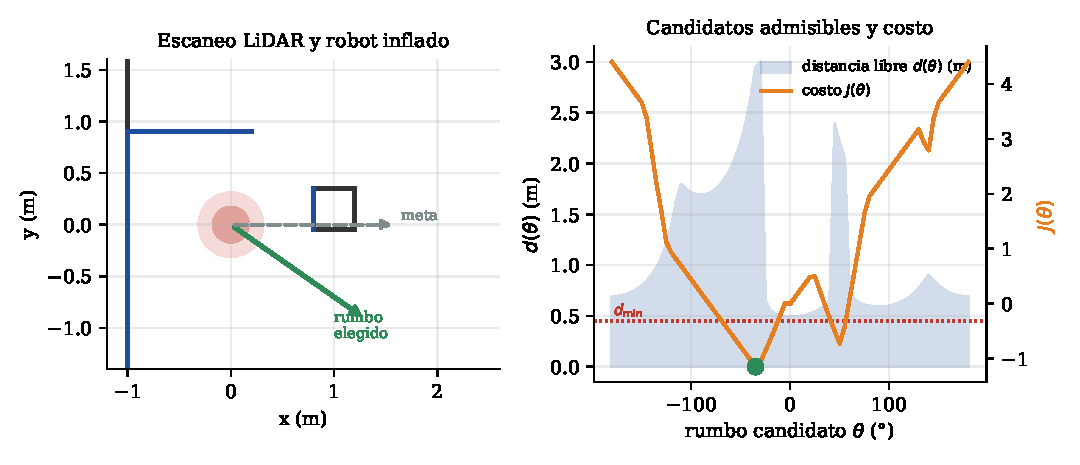
\includegraphics[width=0.95\textwidth]{seleccion_rumbo.pdf}
\caption{Selecci\'on de rumbo en un escaneo simulado. Izquierda: puntos del LiDAR, robot (rojo oscuro) y su versi\'on inflada (rojo claro); la flecha verde es
el rumbo elegido y la gris la direcci\'on de la meta. Derecha: distancia libre $d(\theta)$ por rumbo y costo $J(\theta)$; el punto verde es el m\'inimo entre los rumbos admisibles.}
\label{fig:rumbo}
\end{figure}

\paragraph{Velocidad suave.} La velocidad lineal baja de forma continua con el error angular, $\text{turn\_scale}=\max\!\big(0,\tfrac{\cos\theta-\cos 60^\circ}{1-\cos 60^\circ}\big)$,
en lugar de cortarse de golpe a $60^\circ$; tambi\'en baja cerca de obst\'aculos ($\texttt{slow\_dist}=0.90$~m) y de la meta. Adem\'as limitamos la
aceleraci\'on: $\Delta v\in[-a_{\text{dec}}\Delta t,\,a_{\text{acc}}\Delta t]$ y $\Delta\omega\in[-\alpha\Delta t,\alpha\Delta t]$ con $a_{\text{acc}}=0.35$,
$a_{\text{dec}}=0.8$~m/s$^2$ y $\alpha=2.2$~rad/s$^2$. No es un capricho est\'etico: los arranques bruscos hacen patinar las ruedas y eso arruina la odometr\'ia que usaremos para volver.

\paragraph{Defensa en capas contra choques.}
(1)~Inflado de obst\'aculos; (2)~si el frente libre es menor que la distancia de parada se anula la traslaci\'on y solo se gira en sitio; (3)~el frenado puede ser
m\'as fuerte que la aceleraci\'on; (4)~\emph{bumper}: ante contacto, el robot aborta, retrocede de forma controlada y deja un obst\'aculo virtual en la boca del bloqueo
(as\'i recuerda objetos bajos que el LiDAR no ve); (5)~guardi\'an frontal en la Tarea~B.

\paragraph{Atascos y trampas en U.} Un m\'etodo reactivo puro puede quedar atrapado en m\'inimos locales. Lo mitigamos con un monitor de progreso (si no avanza 8~cm en
\texttt{stuck\_time}$=4.5$~s dispara una maniobra de escape), obst\'aculos virtuales deduplicados con un \emph{k-d tree} 2D propio (sin \texttt{scipy}, para no depender de
paquetes pesados en la Pi) y un detector de concavidades que, si la meta queda dentro de una ``U'' a menos de $0.75$~m, obliga a rodear antes de meterse.

\subsection{Parada y escaneo en $B$}
Declaramos llegada cuando la distancia odom\'etrica a $B$ es menor que \texttt{goal\_tol}$=0.25$~m. El robot frena con la rampa y la m\'aquina de estados pasa a
\textsc{Escanear}: se decodifica la c\'amara, se acumulan cuadros con cara y se aplica el pipeline de la Secci\'on~\ref{sec:facial}. En la Tarea~B el operador dispara el escaneo con la ``V'' mantenida
1.5~s. Al obtener el resultado, el buzzer del Create~3 suena y el nombre se publica en \cmd{/nombre\_reconocido}.

\subsection{Regreso $B\to A$ compensando la deriva}
\label{sec:retorno}
\paragraph{Migas de pan.} En la ida guardamos la pose cada 20~cm. En el regreso las recorremos al rev\'es con un selector que, si hay l\'inea libre hacia una miga m\'as cercana a $A$,
salta directo a ella (atajo). Los callejones sin salida se \emph{podan}: no se vuelve a entrar en ellos. La gran ventaja es que el camino de vuelta ya lo recorrimos hace minutos, as\'i
que sabemos que es transitable; no hay que replanificar sobre un mapa incompleto.

\paragraph{ICP contra la deriva.} La odometr\'ia acumula error. Cada 80~cm de la ida guardamos un \emph{keyframe} (la nube del LiDAR). Al regresar, cuando pasamos cerca de uno, alineamos el
escaneo actual contra \'el minimizando
\[
  E(R,\mathbf{t})=\sum_j \big\lVert \mathbf{q}_j-(R\,\mathbf{p}_j+\mathbf{t})\big\rVert^2 ,
\]
y solo aceptamos la correcci\'on si es confiable ($>60$\,\% de \emph{inliers}, RMSE $<5$~cm y un salto razonable). As\'i corregimos la pose sin necesitar AMCL ni SLAM. En
la Secci\'on~\ref{sec:res-sim} medimos cu\'anto ayuda.

\subsection{La m\'aquina de estados de la misi\'on}
\begin{figure}[H]
\centering
\begin{tikzpicture}[est/.style={draw,circle,align=center,font=\scriptsize,minimum size=16mm,inner sep=1pt,fill=blue!8},
  lbl/.style={font=\scriptsize,above,midway}]
\node[est] (e)   at (0,0)    {ESPERA};
\node[est] (ab)  at (3.6,0)  {IR\_A\_B};
\node[est] (esc) at (7.2,0)  {ESCA-\\NEAR};
\node[est] (ba)  at (10.8,0) {VOLVER\\A\_A};
\node[est] (an)  at (10.8,-3.6) {ANUN-\\CIAR};
\node[est] (fin) at (7.2,-3.6) {FIN};
\node[est,fill=red!15] (par) at (3.6,-3.6) {PARADA};
\draw[flecha] (e)--node[lbl]{sensores OK}(ab);
\draw[flecha] (ab)--node[lbl]{lleg\'o a $B$}(esc);
\draw[flecha] (esc)--node[lbl]{nombre}(ba);
\draw[flecha] (ba)--node[right,font=\scriptsize]{en $A$}(an);
\draw[flecha] (an)--(fin);
\draw[flecha] (ab) to[loop above,looseness=5,min distance=8mm] node[above,font=\scriptsize]{atasco / bumper: escape}(ab);
\draw[flecha] (esc) to[loop above,looseness=5,min distance=8mm] node[above,font=\scriptsize]{sin cara: barrido}(esc);
\draw[flecha,red!60!black,dashed] (ab)--(par);
\draw[flecha,red!60!black,dashed] (esc.south west)--(par.north east);
\draw[flecha,red!60!black,dashed] (ba.south west) to[bend left=12] (par.east);
\node[font=\scriptsize,red!60!black,align=center] at (1.6,-3.6) {emergencia\\o $t>t_{\max}$};
\end{tikzpicture}
\caption{Ciclo de vida de la misi\'on. \textsc{Parada} se alcanza desde cualquier estado activo por parada de emergencia o al superar $t_{\max}$.}
\end{figure}
\begin{description}[nosep,leftmargin=2.3cm,style=sameline]
\item[ESPERA] valida que \cmd{/scan}, \cmd{/odom} y la c\'amara est\'en frescos, fija la pose $A$ y el keyframe~0. En la Tarea~B espera la palma de armado, que adem\'as arranca el cron\'ometro.
\item[IR\_A\_B] navegaci\'on reactiva; migas cada 20~cm y keyframes cada 80~cm.
\item[ESCANEAR] frena, junta cuadros, identifica; si no ve cara, barre.
\item[VOLVER\_A\_A] migas con atajos y correcci\'on ICP.
\item[ANUNCIAR] dice el nombre en $A$ y lo publica. \textbf{FIN} cierra el cron\'ometro y escribe un reporte JSON.
\item[PARADA] anula cualquier comando; por emergencia o por superar $t_{\max}=300$~s.
\end{description}
Para los circuitos con se\~nales, la decisi\'on en cruces es una funci\'on pura (sin ROS ni OpenCV) con prioridad expl\'icita: \emph{llegada} $>$ \emph{hito} $>$ \emph{prohibido} $>$ \emph{flechas} $>$
\emph{rama menos visitada}; y el LiDAR siempre prevalece sobre una se\~nal que contradiga la f\'isica del entorno (por ejemplo, una flecha que apunta a una pared).

%=====================================================================
\section{Justificaci\'on de modelos, algoritmos y decisiones}
\label{sec:just}
%=====================================================================
\subsection{Navegaci\'on: VFH-lite reactivo en lugar de Nav2\,+\,SLAM}
La opci\'on est\'andar en ROS~2 es \texttt{slam\_toolbox} con Nav2 (planificador global y controlador MPPI/DWB). La probamos y la descartamos; la Tabla~\ref{tab:nav} resume por qu\'e.

\begin{table}[H]
\centering\small
\begin{tabularx}{\textwidth}{@{}>{\raggedright\arraybackslash}p{3.0cm}>{\raggedright\arraybackslash}X>{\raggedright\arraybackslash}X@{}}
\toprule
\textbf{Criterio} & \textbf{VFH-lite + migas + ICP (elegido)} & \textbf{Nav2 + SLAM Toolbox} \\
\midrule
CPU en la Pi 4 & $\approx$25\,\% de un n\'ucleo (solo retransmite) & Satura los 4 n\'ucleos \\
Latencia de decisi\'on & $<1$~ms por ciclo (NumPy vectorizado) & 40--120~ms; \cmd{cmd\_vel} cae bajo 5~Hz \\
Obst\'aculos nuevos & Reacci\'on inmediata (se recalculan los rumbos en cada escaneo) & Debe inflarse en el costmap y replanificar \\
Dependencia del reloj & Tolerante (navegaci\'on relativa) & Cr\'itica: desfase $\ge1$~s descarta \emph{scans} \\
Pasillos de $\sim$80~cm & Fluido, centrado por margen lateral & Entra en \emph{recovery} (giros en sitio) \\
Regreso & Determinista: camino ya verificado & Nueva ruta global en mapa incompleto \\
Memoria & $<60$~MB & $>1.2$~GB en la Pi \\
Optimalidad global & Limitada en laberintos profundos & Superior con mapa completo \\
\bottomrule
\end{tabularx}
\caption{Comparaci\'on de estrategias de navegaci\'on. Las cifras provienen de las pruebas del equipo en el laboratorio; no las repetimos de forma controlada para este informe.}
\label{tab:nav}
\end{table}

\begin{decision}{Por qu\'e aceptamos perder optimalidad}
El \'unico costo real de nuestra elecci\'on es que no buscamos el camino m\'as corto global. Lo aceptamos porque la m\'etrica premia la \emph{confiabilidad}: en un circuito corto y
desconocido, reaccionar r\'apido y volver por un camino que ya sabemos libre gana m\'as puntos que un plan \'optimo que depende de un mapa que no tenemos.
\end{decision}

\subsection{Visi\'on facial: YuNet\,+\,SFace}
\begin{itemize}
\item \textbf{Ligero y offline}: ambos modelos son ONNX y corren en CPU con OpenCV DNN, sin GPU ni internet. YuNet detecta en 13--16~ms por imagen en la laptop.
\item \textbf{Alternativa que evaluamos}: un modelo de embedding afinado (tipo AdaFace, 512 dimensiones, 261~MB) discrimina m\'as, pero en hardware modesto tarda de 0.7 a 1.9~s por cara solo
en el embedding (de 8 a 27~s en Windows), y no podemos verificar con qui\'en fue afinado. Lo dejamos como verificador as\'incrono opcional, fuera del lazo cr\'itico.
\item \textbf{Precisi\'on vs.\ latencia}: elegimos el descriptor r\'apido y recuperamos precisi\'on con trucos baratos: fusi\'on de los $K=3$ mejores cuadros, galer\'ia con espejo, margen
sobre el segundo y filtro de nitidez.
\item \textbf{Umbral}: $\tau=0.363$ es el valor gen\'erico de OpenCV, no uno calibrado con nuestra galer\'ia. Calibrarlo con fotos nuevas es la mejora de mayor valor pendiente.
\end{itemize}

\subsection{Gestos: reglas geom\'etricas sobre MediaPipe}
Preferimos reglas angulares y de distancia relativa sobre los landmarks antes que entrenar un clasificador: no necesitan datos etiquetados, son interpretables y se depuran en el laboratorio,
y son invariantes a la escala gracias a la normalizaci\'on con $s$. El costo es sensibilidad a poses ambiguas; lo compensamos con el filtrado temporal y el armado expl\'icito. Un clasificador aprendido
ser\'ia m\'as robusto entre operadores, pero exigir\'ia datos y tiempo que no ten\'iamos.

\subsection{Velocidad frente a riesgo de colisi\'on}
Como $t$ incluye penalizaciones y fallar vale cero, elegimos valores conservadores: $v_{\max}=0.14$~m/s (el Create~3 puede llegar a 0.31), margen de seguridad $0.14$~m en vez de $0.09$ y
$d_{\text{stop}}=0.38$~m. Para elegirlos de forma sistem\'atica tenemos \cmd{calibrar.py}: para N intentos por juego de par\'ametros calcula el costo $C = t + c\cdot n_{\text{choques}} + e\cdot n_{\text{id. err\'oneas}}$ y
nos quedamos con el menor.

\begin{figure}[H]
\centering
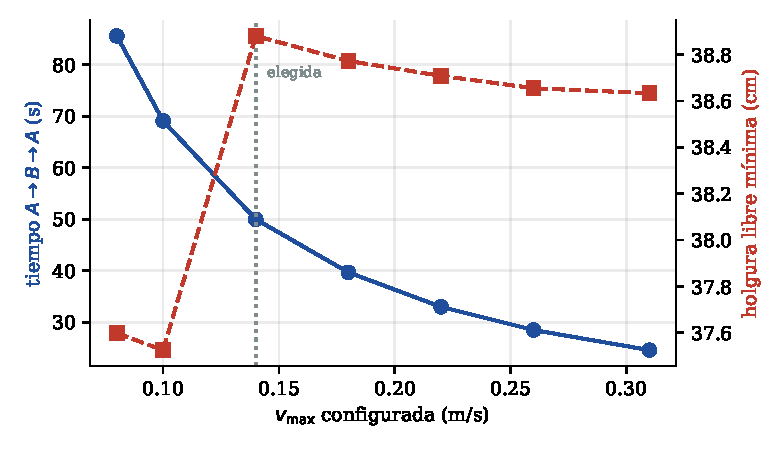
\includegraphics[width=0.62\textwidth]{velocidad.pdf}
\caption{Tiempo de misi\'on y holgura m\'inima a las paredes frente a la velocidad m\'axima, en el simulador (circuito de obst\'aculos en sala). El tiempo cae casi como $1/v$; la holgura no se mueve porque \textbf{el simulador no modela patinaje, latencia ni ruido}, que es de donde viene el riesgo real a velocidad alta.}
\label{fig:vel}
\end{figure}

\begin{alerta}{Ojo con lo que dice esta figura}
La simulaci\'on confirma la mitad del compromiso: ir de $0.31$ a $0.14$~m/s multiplica el tiempo por unas 2 veces (de 24.6~s a 50.0~s). La otra mitad, el aumento del riesgo de choque con la
velocidad, \emph{no} se puede ver en este simulador. Sigue sustentado en lo que observamos en el robot (patinaje y odometr\'ia degradada) y ser\'a validado con \cmd{calibrar.py} en pista real.
\end{alerta}

%=====================================================================
\section{Resultados experimentales y an\'alisis de rendimiento}
\label{sec:result}
%=====================================================================
Dividimos la evidencia en tres niveles para no mezclar peras con manzanas (Tabla~\ref{tab:evidencia}).

\begin{table}[H]
\centering\small
\begin{tabularx}{\textwidth}{@{}>{\raggedright\arraybackslash}p{3.7cm}>{\raggedright\arraybackslash}X@{}}
\toprule
\textbf{Nivel} & \textbf{Qu\'e contiene} \\
\midrule
Robot f\'isico (laboratorio) & Salud del sistema, frecuencias de sensores, sincronizaci\'on de reloj (Secci\'on~\ref{sec:res-hw}). \\
Simulador + pruebas unitarias & Misiones completas $A\to B\to A$ con el c\'odigo real de navegaci\'on, efecto del ICP, sensibilidad a la velocidad, 192 pruebas aprobadas (Secci\'on~\ref{sec:res-sim}). \\
\pend{pendiente} & Tiempos y choques en pista real, precisi\'on facial con galer\'ia real, latencia de gestos (Secci\'on~\ref{sec:res-pend}). \\
\bottomrule
\end{tabularx}
\caption{Niveles de evidencia de este informe.}
\label{tab:evidencia}
\end{table}

\subsection{Pruebas de hardware y enlace (robot f\'isico)}
\label{sec:res-hw}
Con Ethernet directo y \texttt{turtlebot4.service} activo en reposo medimos:
\begin{table}[H]
\centering\small
\begin{tabular}{@{}lr@{}}
\toprule
\textbf{M\'etrica} & \textbf{Valor medido} \\
\midrule
Carga de CPU de la Pi (load average) & 0.95 ($\approx$24\,\% de capacidad) \\
Temperatura de la Pi & 55.5\,\textdegree C, sin \emph{throttling} (\texttt{throttled=0x0}) \\
Frecuencia LiDAR / odometr\'ia / IMU & 7.6 / 17.2 / 32.8~Hz \\
C\'amara OAK-D (vista previa) & 24.6~FPS, enlace USB~3 SuperSpeed \\
Desfase de reloj entre sensores & 75\,368~s $\to$ 0.08~s tras reiniciar NTP del Create~3 \\
Latencia del enlace laptop--robot & $<1$~ms (Ethernet directo) \\
\bottomrule
\end{tabular}
\caption{Medidas en el laboratorio.}
\end{table}

\subsection{Simulaci\'on: el c\'odigo real de navegaci\'on, misi\'on completa}
\label{sec:res-sim}
No quisimos que la secci\'on de resultados dependiera solo de pruebas unitarias, as\'i que escribimos un script (\cmd{generar\_figuras.py}) que ejecuta el \emph{mismo} \cmd{Piloto} del robot sobre un simulador de
LiDAR con trazado de rayos y una odometr\'ia que puede derivar, usando los par\'ametros de \cmd{config.json}. Todos los n\'umeros y figuras de esta secci\'on salen de ese script; si cambiamos la configuraci\'on
se regeneran. La suite de pruebas del repositorio tambi\'en pasa: \textbf{192 pruebas aprobadas, 1 omitida} (ejecutadas el 15 de noviembre de 2026).

\paragraph{Cuatro circuitos.} La Figura~\ref{fig:tray} muestra las trayectorias y la Tabla~\ref{tab:circ} las m\'etricas. En tres de los cuatro circuitos el robot completa $A\to B\to A$ sin ning\'un choque
(en el simulador, ``choque'' es que el disco del robot toque una pared). Incluye un laberinto con callej\'on sin salida y un obst\'aculo bajo que el LiDAR no ve y s\'olo se detecta por el bumper simulado.

\begin{figure}[H]
\centering
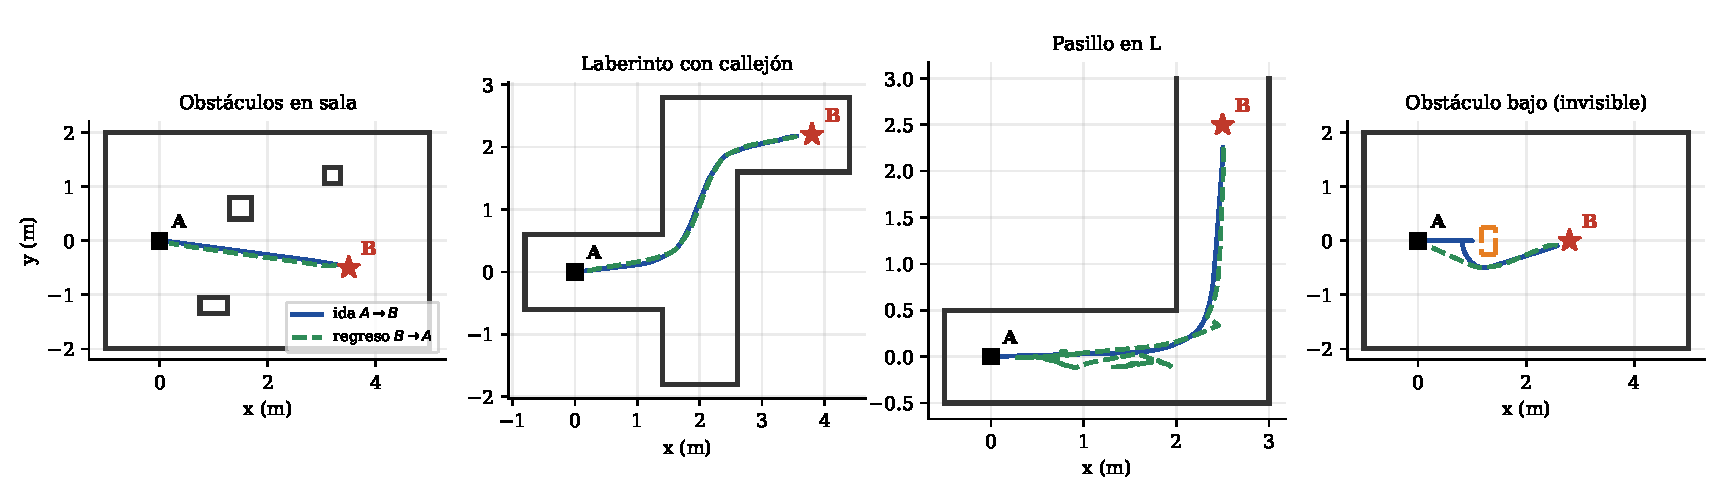
\includegraphics[width=\textwidth]{trayectorias.pdf}
\caption{Trayectorias en simulaci\'on con la configuraci\'on final. Azul: ida; verde discontinuo: regreso; l\'inea naranja discontinua: obst\'aculo que el LiDAR no ve. En el pasillo en L (tercero) el robot no completa la misi\'on; se discute en la Secci\'on~\ref{sec:futuro}.}
\label{fig:tray}
\end{figure}

\begin{table}[H]
\centering\small
\TablaCircuitos
\caption{Resultados por circuito (simulaci\'on, un intento por circuito, configuraci\'on final). ``Holgura'' es la distancia libre m\'inima entre el borde del robot y la pared. El error en $A$ queda cerca de 20~cm porque el robot se detiene al entrar en la tolerancia \texttt{home\_tol}$=0.20$~m.}
\label{tab:circ}
\end{table}

\paragraph{Perfil de velocidad.} La Figura~\ref{fig:perfil} muestra lo que hace el controlador en el circuito de obst\'aculos: arranque con rampa, reducci\'on al rodear cada obst\'aculo, giros en sitio cuando el rumbo
admisible queda a m\'as de $60^\circ$, y frenado al llegar a $B$.

\begin{figure}[H]
\centering
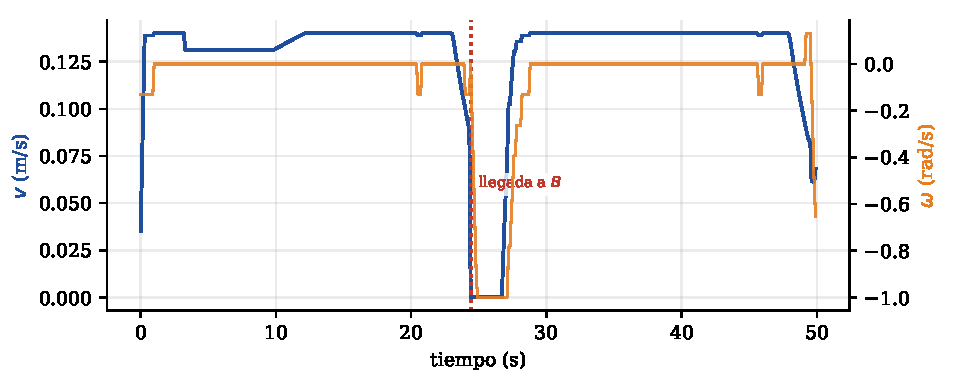
\includegraphics[width=0.8\textwidth]{perfil_velocidad.pdf}
\caption{Comandos $v$ y $\omega$ durante la misi\'on del circuito de obst\'aculos. La l\'inea roja marca la llegada a $B$.}
\label{fig:perfil}
\end{figure}

\paragraph{El ICP s\'i hace falta.} Para medir la correcci\'on de deriva repetimos cinco misiones (cinco metas distintas) por cada nivel de error de escala en el giro de la odometr\'ia, con y sin ICP (en el modo ``sin ICP'' se descartan todas las correcciones, igual que en
la prueba unitaria del repositorio). El resultado est\'a en la Figura~\ref{fig:deriva} y la Tabla~\ref{tab:deriva}: sin ICP el error al volver crece casi linealmente con la deriva y supera la tolerancia desde el 4\,\%; con ICP queda siempre
dentro de la tolerancia, incluso con 12\,\% de error.

\begin{figure}[H]
\centering
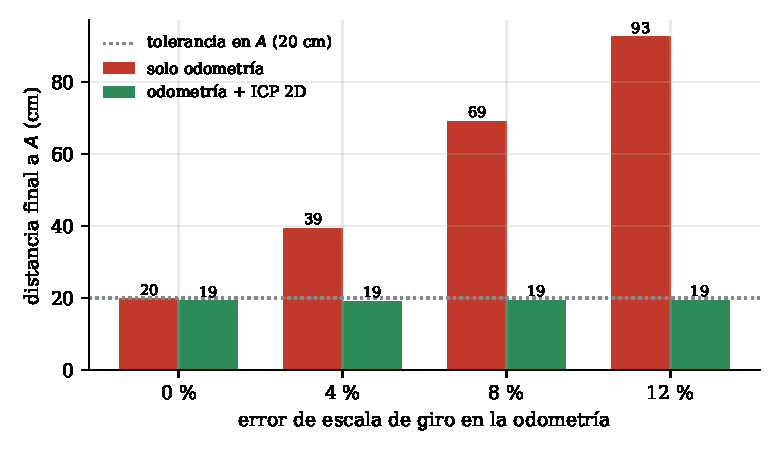
\includegraphics[width=0.62\textwidth]{deriva_icp.pdf}
\caption{Distancia final a $A$ (media de 5 misiones) seg\'un el error de escala del giro en la odometr\'ia, con y sin correcci\'on ICP.}
\label{fig:deriva}
\end{figure}

\begin{table}[H]
\centering\small
\TablaDeriva
\caption{Efecto del ICP en la deriva (5 metas por celda, circuito de obst\'aculos en sala).}
\label{tab:deriva}
\end{table}

\paragraph{Velocidad.} La Tabla~\ref{tab:vel} detalla la curva de la Figura~\ref{fig:vel}; sin choques en ning\'un caso, pero recordemos que el simulador no representa el riesgo real a alta velocidad.
\begin{table}[H]
\centering\small
\TablaVelocidad
\caption{Tiempo de misi\'on frente a $v_{\max}$ (simulaci\'on).}
\label{tab:vel}
\end{table}

\paragraph{Lo que la simulaci\'on no puede decirnos.} El simulador usa escaneos ideales (sin ruido ni rayos perdidos), un robot que no patina y comunicaci\'on sin latencia. Los resultados validan la \emph{l\'ogica} (decisi\'on, memoria, ICP) pero
no sustituyen las pruebas en pista con el robot real.

\subsection{Resultados pendientes de medir}
\label{sec:res-pend}
Estas tablas se llenar\'an con las sesiones en el laboratorio y con el ensayo general (un circuito que nadie haya visto, tres intentos por tarea). Ya tienen la forma final.

\begin{table}[H]
\centering\small
\begin{tabular}{@{}lcccc@{}}
\toprule
\textbf{Intento} & \textbf{Tarea} & \textbf{$t$ (s)} & \textbf{Choques} & \textbf{Regres\'o y nombre OK} \\
\midrule
1 & A & \pend{} & \pend{} & \pend{} \\
2 & A & \pend{} & \pend{} & \pend{} \\
3 & A & \pend{} & \pend{} & \pend{} \\
1 & B & \pend{} & \pend{} & \pend{} \\
2 & B & \pend{} & \pend{} & \pend{} \\
3 & B & \pend{} & \pend{} & \pend{} \\
\bottomrule
\end{tabular}
\caption{Tiempos y penalizaciones en el ensayo general (por medir).}
\end{table}

\begin{table}[H]
\centering\small
\begin{tabular}{@{}lc@{}}
\toprule
\textbf{M\'etrica de visi\'on y gestos} & \textbf{Valor} \\
\midrule
Precisi\'on top-1 (galer\'ia real, foto impresa con la c\'amara del robot) & \pend{\%} \\
Precisi\'on deja-uno-fuera (\cmd{facial.py --probar}) & \pend{\%} \\
Confusiones con resultado ``seguro'' & \pend{n} \\
Fotos sin cara detectada & \pend{\%} \\
Latencia de identificaci\'on (mediana / p95) & \pend{ms} \\
Latencia gesto $\to$ \cmd{cmd\_vel} (mediana) & \pend{ms} \\
Falsos positivos de gesto por minuto & \pend{n} \\
Deriva real de odometr\'ia en $A\to B\to A$ (con / sin ICP) & \pend{cm} \\
Robustez ante iluminaci\'on (buena / baja / contraluz) & \pend{\%} \\
\bottomrule
\end{tabular}
\caption{M\'etricas de visi\'on y gestos por obtener.}
\end{table}

%=====================================================================
\section{Limitaciones y trabajo futuro}
\label{sec:futuro}
%=====================================================================
\subsection{Un fallo real: el pasillo en L}
\begin{alerta}{Lo que encontramos al escribir este informe}
Con la configuraci\'on conservadora final, el robot \textbf{no completa} en el simulador un pasillo en L de 1~m de ancho, aunque no choca: se queda dando vueltas hasta agotar el tiempo (200~s en esta prueba).
Ese mismo circuito s\'i lo resuelve la prueba unitaria del repositorio (72.8~s) porque usa los par\'ametros por defecto. La Tabla~\ref{tab:L} aisla qu\'e par\'ametros lo provocan.
\end{alerta}

\begin{table}[H]
\centering\small
\begin{tabular}{@{}lcc@{}}
\toprule
\textbf{Configuraci\'on} & $v_{\max}=0.20$ & $v_{\max}=0.14$ \\
\midrule
Por defecto & completa (72.8~s) & \textcolor{rojo}{no completa} \\
\texttt{wall\_min}\,=\,0.38 & completa (71.9~s) & \textcolor{rojo}{no completa} \\
\texttt{stop\_dist}\,=\,0.38 & \textcolor{rojo}{no completa} & \textcolor{rojo}{no completa} \\
\texttt{safety\_margin}\,=\,0.14 & \textcolor{rojo}{no completa} & \textcolor{rojo}{no completa} \\
Configuraci\'on final (\texttt{config.json}) & \textcolor{rojo}{no completa} & \textcolor{rojo}{no completa} \\
\bottomrule
\end{tabular}
\caption{Sensibilidad del pasillo en L (simulaci\'on, l\'imite de 200~s, sin choques en ning\'un caso).}
\label{tab:L}
\end{table}

Lo que se ve es una tensi\'on real entre \emph{seguridad} y \emph{espacio disponible}: con $R_{\text{inf}}=0.31$~m el disco inflado deja poco margen en un pasillo de 1~m (el lab tiene tramos de unos 80~cm), y bajar la velocidad
tambi\'en rompe el caso. No lo depuramos todav\'ia; es la primera tarea antes del ensayo general: encontrar por qu\'e velocidades menores impiden la curva (hip\'otesis: interacci\'on entre el monitor de atascos, el
margen lateral y la rampa de aceleraci\'on) y repetir la prueba con \cmd{calibrar.py}.

\subsection{Otras limitaciones}
\begin{itemize}
\item \textbf{Iluminaci\'on}: YuNet/SFace y MediaPipe se degradan con contraluz o poca luz; la foto impresa agrega brillo especular y baja resoluci\'on efectiva.
\item \textbf{Deriva de odometr\'ia}: depende del piso; el ICP corrige solo si hay estructura geom\'etrica suficiente (en pasillos largos y lisos el problema es degenerado a lo largo del eje).
\item \textbf{LiDAR 2D}: ve solo un plano; los obst\'aculos bajos quedan para el bumper y no hay percepci\'on trasera. El alcance y los $\sim$7.6~Hz limitan la velocidad segura.
\item \textbf{Reactividad sin visi\'on global}: en laberintos con callejones profundos puede perder tiempo y no hay garant\'ia de completitud (el laberinto simulado tard\'o 104~s).
\item \textbf{Galer\'ia peque\~na y umbral gen\'erico}: con pocas fotos por persona, compa\~neros parecidos tienen poco margen; $\tau$ no est\'a calibrado.
\item \textbf{Dependencia del enlace} en la modalidad laptop: un corte de red detiene el control. La modalidad \emph{edge} lo mitiga pero a\'un no se valid\'o en pista.
\item \textbf{Estado de validaci\'on}: la navegaci\'on y los gestos se probaron en simulador y con gestos sint\'eticos; falta la validaci\'on integral en pista.
\end{itemize}

\subsection{Mejoras propuestas, por orden de valor}
\begin{enumerate}
\item Depurar el caso del pasillo en L y fijar una configuraci\'on que sea segura \emph{y} complete circuitos estrechos (barrido de par\'ametros con \cmd{calibrar.py}).
\item Fotos de prueba \emph{no vistas} para calibrar $\tau$ y $\delta$ con matriz de confusi\'on.
\item Galer\'ia aumentada con efectos de foto impresa (desenfoque, perspectiva, brillo, JPEG).
\item Cascada de reconocimiento: embedding r\'apido primero y modelo preciso as\'incrono solo si el margen es bajo.
\item Fusionar la \textbf{profundidad de la OAK-D} con el LiDAR para ver obst\'aculos fuera del plano de escaneo.
\item Reemplazar las reglas de gestos por un clasificador ligero entrenado con landmarks (robustez entre operadores).
\item Odometr\'ia visual--inercial como respaldo del ICP en pasillos degenerados.
\item Hacer que el simulador modele patinaje, ruido y latencia, para que el compromiso velocidad--riesgo se pueda estudiar sin el robot.
\end{enumerate}

%=====================================================================
\section{Conclusiones}
%=====================================================================
Dise\~namos el sistema pensando en una sola cosa: llegar y volver sin chocar. Por eso elegimos un navegador reactivo que cabe en la Raspberry~Pi, memoria de camino para el regreso y un ICP que
corrige la odometr\'ia; en simulaci\'on, ese ICP mantiene el error de vuelta en 19--20~cm incluso con 12\,\% de deriva, mientras que sin \'el llega a 92~cm. El pipeline YuNet\,+\,SFace cumple lo que pide la competencia
(offline, r\'apido, galer\'ia cargada en segundos) y los gestos son deliberadamente desconfiados para que ninguna orden dudosa mueva al robot.

Tambi\'en somos claros con lo que falta: no tenemos todav\'ia m\'etricas en pista real, la precisi\'on facial no est\'a medida con la galer\'ia definitiva y hay un circuito estrecho que la configuraci\'on final no resuelve. Esas
tres cosas son nuestro plan para la semana previa a la presentaci\'on.

%=====================================================================
\section*{Referencias}
\addcontentsline{toc}{section}{Referencias}
%=====================================================================
\begin{thebibliography}{9}
\bibitem{vfh} J.~Borenstein, Y.~Koren. \emph{The Vector Field Histogram -- Fast Obstacle Avoidance for Mobile Robots}. IEEE Trans.\ Robotics and Automation, 7(3), 1991.
\bibitem{icp} P.~Besl, N.~McKay. \emph{A Method for Registration of 3-D Shapes}. IEEE TPAMI, 14(2), 1992.
\bibitem{yunet} S.~Wu et al. \emph{YuNet: A Tiny Millisecond-level Face Detector}. Machine Intelligence Research, 2023.
\bibitem{sface} Z.~Zhong et al. \emph{SFace: Sigmoid-Constrained Hypersphere Loss for Robust Face Recognition}. IEEE TIP, 2021.
\bibitem{mp} F.~Zhang et al. \emph{MediaPipe Hands: On-device Real-time Hand Tracking}. arXiv:2006.10214, 2020.
\bibitem{nav2} S.~Macenski et al. \emph{The Marathon 2: A Navigation System}. IROS, 2020.
\end{thebibliography}

%=====================================================================
\appendix
\section{Ap\'endice A: Fragmentos de c\'odigo relevantes}
%=====================================================================
Solo los fragmentos clave; el c\'odigo completo est\'a en el repositorio y en la carpeta compartida.

\subsection{Calidad de cuadro y decisi\'on facial (\texttt{facial.py})}
\begin{lstlisting}
def calidad(img, face):
    x, y, w, h = (int(v) for v in face[:4])
    crop = img[max(y, 0):y + h, max(x, 0):x + w]
    sharp = cv2.Laplacian(cv2.cvtColor(crop, cv2.COLOR_BGR2GRAY), cv2.CV_64F).var()
    return float(face[14] * min(w / 80.0, 1.0) * min(sharp / 100.0, 1.0))

def identificar(frames, rostros, galeria, umbral=0.363, margen=0.04, top=3):
    cands = []
    for f in frames:
        img, faces = rostros.detectar(f)
        if len(faces):
            cands.append((calidad(img, faces[0]), img, faces[0]))
    cands.sort(key=lambda c: -c[0])
    sims = np.mean([galeria.similitudes(rostros.embedding(img, face))
                    for _, img, face in cands[:top]], axis=0)
    order = np.argsort(-sims)
    segundo = sims[order[1]] if len(order) > 1 else -1.0
    seguro = sims[order[0]] >= umbral and sims[order[0]] - segundo >= margen
\end{lstlisting}

\subsection{Selecci\'on de rumbo (\texttt{nav\_core.py})}
\begin{lstlisting}
def choose_heading(ranges, angles, goal, prev=0.0, p=NavParams(), avoid_concavity=False):
    hs = headings(p)                                   # 73 rumbos, cada 5 grados
    free = free_distance(ranges, angles, hs, p)        # disco inflado
    ok = free >= p.min_free
    if not ok.any():
        return None
    margin = side_margin(ranges, angles, hs, p)
    cost = (p.w_goal * np.abs(wrap(hs - goal))
            + p.w_turn * np.abs(wrap(hs - prev))
            - p.w_clear * margin)
    cost = np.where(ok, cost, np.inf)
    return float(hs[np.argmin(cost)])
\end{lstlisting}

\subsection{M\'aquina de armado de gestos (\texttt{gestos\_teleop.py})}
\begin{lstlisting}
def update(self, pose, t):
    self.count = self.count + 1 if pose == self.last else 1
    self.last = pose
    stable = pose if self.count >= self.stable else None     # >= 3 cuadros
    if stable != self.held:
        self.held, self.held_t0, self.fired = stable, t, False
    held_for = t - self.held_t0
    if stable == "puno" and self.armed:
        self.armed, evento = False, "desarmado"
    elif stable == "palma" and not self.armed and held_for >= self.arm_hold:
        self.armed, self.fired, evento = True, True, "armado"
    elif stable == "victoria" and self.armed and held_for >= self.action_hold:
        self.fired, evento = True, "accion"
    direction = POSES[stable][1] if self.armed and stable in POSES else (0, 0)
\end{lstlisting}

\subsection{Decisi\'on en cruces (\texttt{decision.py}, resumen)}
\begin{lstlisting}
def decidir(opciones, senal=None, visitado=None, ...):
    libres = set(opciones)
    if tipo == "bandera":   return "llegada_b"
    if tipo == "prohibido": bloqueadas.add("recto")           # rama agotada
    disponibles = libres - bloqueadas
    if tipo in ("izq", "der") and tipo in disponibles: return tipo
    if not disponibles:     return "retroceder"               # callejon
    return min(disponibles, key=lambda op: (visitas(op), pref[op], op))
\end{lstlisting}

\section{Ap\'endice B: Par\'ametros finales (\texttt{config.json})}
\begin{table}[H]
\centering\small
\begin{tabularx}{\textwidth}{@{}ll>{\raggedright\arraybackslash}X@{}}
\toprule
\textbf{Par\'ametro} & \textbf{Valor} & \textbf{Significado} \\
\midrule
\texttt{max\_linear} & 0.14 m/s & Velocidad lineal m\'axima \\
\texttt{max\_angular} & 1.0 rad/s & Velocidad angular m\'axima \\
\texttt{max\_accel / max\_decel} & 0.35 / 0.8 m/s$^2$ & Rampas lineales \\
\texttt{max\_alpha} & 2.2 rad/s$^2$ & Rampa angular \\
\texttt{safety\_margin} & 0.14 m & Margen de inflado sobre $R_{\text{robot}}=0.17$ \\
\texttt{stop\_dist / slow\_dist} & 0.38 / 0.90 m & Parada y reducci\'on de velocidad \\
\texttt{wall\_min} & 0.38 m & Distancia m\'inima a paredes \\
\texttt{goal\_tol / home\_tol} & 0.25 / 0.20 m & Tolerancia de llegada a $B$ / $A$ \\
\texttt{stuck\_time} & 4.5 s & Tiempo sin progreso para activar el escape \\
\texttt{t\_max} & 300 s & L\'imite de la misi\'on \\
\texttt{regreso\_modo} & migas & Estrategia de retorno \\
\bottomrule
\end{tabularx}
\end{table}

\section{Ap\'endice C: Configuraci\'on de red}
\begin{lstlisting}[language=bash]
# En WSL, con el robot conectado (Wi-Fi 192.168.0.104 o cable 192.168.185.3)
source ~/turtleclaude4/tb4_connect.sh 192.168.0.104 67
export FASTRTPS_DEFAULT_PROFILES_FILE=~/turtleclaude4/fastdds_pc.xml   # peers estaticos
./tb4_check.sh 192.168.0.104        # verifica /scan, /odom, camara y reloj
\end{lstlisting}

\section{Ap\'endice D: C\'omo reproducir las figuras de simulaci\'on}
\begin{lstlisting}[language=bash]
cd entregables/informe_tecnico
python generar_figuras.py     # corre el Piloto real en el simulador (~3 min)
pdflatex informe.tex && pdflatex informe.tex
\end{lstlisting}

\end{document}
